\section{Stmívaný zdroj světla}
K budíku lze připojit zdroj světla (ve firmware je tato funkce nazývána
\texttt{ambient}), který je pozvolna rozsvěcen před zahájením akustického
buzení. Cílem je simulovat postupné rozednění.

Na výstupu \MCUpin{PD6} mikrokontroléru je PWM signál o frekvenci
\SI{980}{\hertz}\footnote{\url{https://www.arduino.cc/reference/en/language/functions/analog-io/analogwrite/}}.
Na většině ostatních výstupních pinů by byla frekvence \SI{490}{\hertz}, piny 5
a 6 jsou v tomto výjimečné. % Pouze uno, na MEGA piny 4 a 13
Přímé řízení samostatné výkonové LED či LED pásku tímto signálem by způsobovalo
blikání světla na této frekvenci. Proto je vhodnější plynule regulovat proud
protékající LED, která je napájena zdrojem konstantního proudu.
% https://electronics.stackexchange.com/questions/277238/disadvantages-of-dimming-leds-via-current-regulation-as-opposed-to-via-pulse-fre


\subsection{Testovací verze}
Pro prvotní ověření užitečnosti celého konceptu byl vytvořen jednoduchý
tranzistorový obvod, který slouží k napájení jedné LED o jmenovitém výkonu
\SI{1}{\watt} ze zdroje o napětí \SI{12}{\volt}. Obvod je určen pouze pro
testování a při jeho návrhu proto nebylo věnováno příliš pozornosti tomu, aby
byla závislost proudu protékajícího LED na střídě PWM signálu lineární (viz
graf na obrázku~\vref{fig:ambient linear testing sim napeti}).
Z tohoto důvodu není obvod vhodný pro použití ve finálním výrobku. Dalšími
nevýhodami jsou nízká účinnost, potřeba chladit výkonový tranzistor a z toho
vyplývající velké fyzické rozměry součástek. Obvod ale lze velmi snadno
sestavit na nepájivém kontaktním poli.

Výkonovou LED v pouzdře pro povrchovou montáž je nutné chladit, pro testování
prototypů lze využít výrobcem dodaný chladič. Jde o malou desku plošných spojů
s hliníkovým podkladem. Pro odvod tepla má LED na spodní straně plochu pro
připájení k chladiči. To znemožňuje pájení standardní mikropáječkou, spodní
strana totiž není přístupná. Vhodnější metodou je aplikování pájecí pasty
(tavidlo s obsahem pájky) a zahřátí celé desky na teplotu pájení. Pájení horkým
vzduchem by zbytečně tepelně namáhalo horní stranu LED (např. čočku), proto je
vhodnější aplikovat teplo ze spodní strany.

\begin{figure}[htbp]
    \centering
    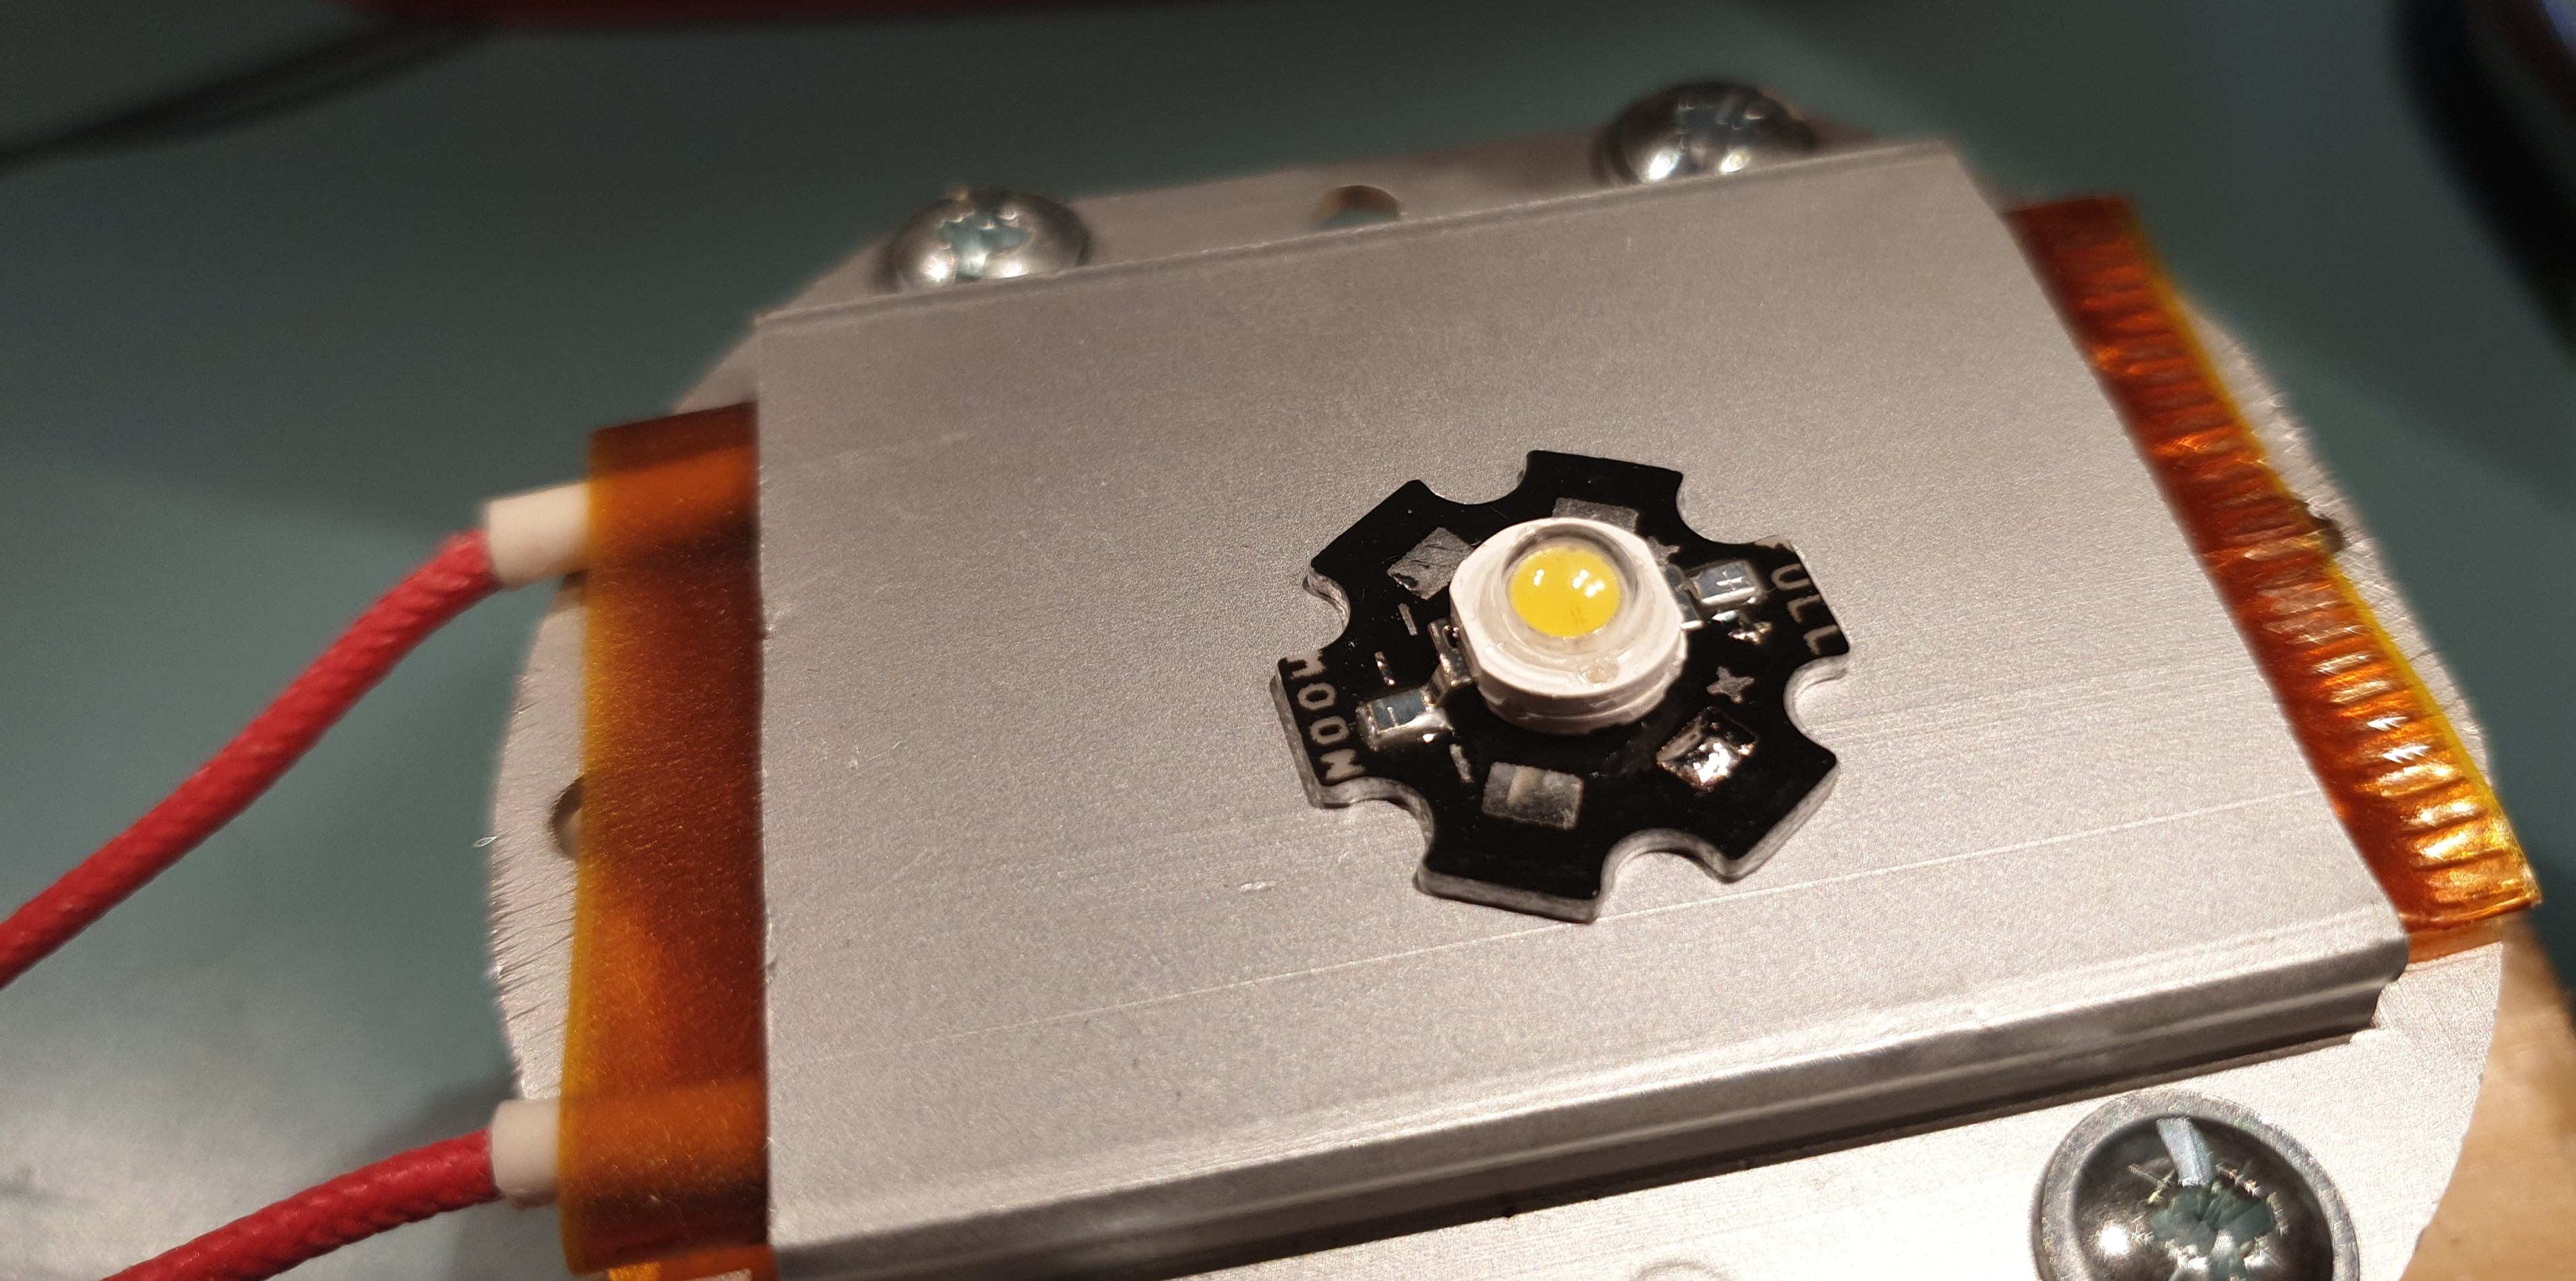
\includegraphics[width=0.6\textwidth]{ambient-LED-pajeni}
    \caption{Pájení výkonové SMD LED na chladič}
    \label{fig:ambient LED pajeni}
\end{figure}



\begin{figure}[htbp]
    \centering
    \includegraphics[width=0.9\textwidth]{cropped_ambient-linear-testing}
    \caption{Schéma zapojení testovacího lineárního stmívače pro výkonovou LED}
    \label{fig:ambient linear testing sch}
\end{figure}

\begin{figure}[htbp]
    \centering
    \subcaptionbox{%
        Schéma zapojení a nastavení simulace%
        \label{fig:ambient linear testing sim sch}
    }{%
        \includegraphics[width=0.9\textwidth]{sim/cropped_ambient-linear-testing}
    }
    \subcaptionbox{%
        Závislost proudu protékajícího LED na napětí zdroje V1 reprezentujícího
        kondenzátor $C_1$ z~obrázku~\vref{fig:ambient linear testing sch}%
        \label{fig:ambient linear testing sim napeti}
    }{%
        \input{sim/graf-ambient-linear-testing.tex}
    }
    \caption{Simulace testovacího lineárního stmívače v programu LTspice}
    \label{fig:ambient linear testing sim}
\end{figure}

Vstupní PWM signál je převáděn na analogové napětí dolní propustí (integračním
článkem RC tvořeným R1 a C1). Rezistory R2 a R3 určují střídu PWM
signálu, při které se LED začne rozsvěcet a kdy dosáhne plného jasu. Tranzistor
Q2 je použit kvůli nízkému proudovému zesilovacímu činiteli tranzistoru Q3, se
kterým tvoří darlingtonovo zapojení. Tranzistor Q3 reguluje proud protékající
LED (D1). Z důvodu poměrně velkého ztrátového výkonu na této součástce byl
použit tranzistor KUY12 v pouzdře TO-3. Rezistor R4 převádí proud protékající
větví s LED na napětí. Velikost odporu tohoto rezistoru určuje konstantní proud
při plném jasu, protože tranzistor Q1 na tomto rezistoru udržuje přibližně
konstantní úbytek napětí ($U_\mathrm{CE} \cong \SI{700}{\milli\volt}$).
Konstantní proud je tedy $I = \frac{U_\mathrm{CE}}{R_4} =
\frac{\SI{700}{\milli\volt}}{\SI{6,8}{\ohm}} \doteq \SI{103}{\milli\ampere}$.
Regulace probíhá přivíráním Q3.

\FloatBarrier
\subsection{Konečná verze}
Na finální verzi stmívače jsou přísnější požadavky:
\begin{itemize}
    \item Obvod musí pracovat při napájecím napětí \SI{5}{\volt}.
    \item Při nulové střídě PWM signálu $d = \SI{0}{\percent}$ musí být LED
        zcela zhasnutá.
    \item Při střídě $d = \SI{100}{\percent}$ musí být proud protékající LED
        udržován konstantní na bezpečné hodnotě, nezávisle na jejím úbytku
        napětí a velikosti napájecího napětí.
    \item Závislost proudu protékajícího LED (a tedy i její svítivosti) na
        střídě PWM signálu musí být přibližně lineární, rozsah
        $\SI{0}{\percent} \le d \le \SI{100}{\percent}$ musí být co nejlépe
        využit při zachování jednoduchosti obvodového řešení.
    \item Tepelné ztráty regulačního obvodu nesmí být příliš velké, aktivní
        i pasivní součástky by se měly obejít bez rozměrných chladičů.
\end{itemize}

Vycházíme z obvodu dle obrázku~\vref{fig:ambient linear testing sch} a dále jej
zdokonalujeme. Aby nedošlo k dosažení maximálního jasu příliš brzy, můžeme
zvýšit napětí na rezistoru R4, při kterém dochází k omezování proudu. Toho lze
dosáhnout přidáním polovodičové diody D2 v propustném směru mezi emitor Q1
a~zem. Střídu, při které se začne LED rozsvěcet, můžeme zmenšit přidáním
rezistoru mezi zdroj napětí \SI{5}{\volt} a bázi Q2. Nechtěným oscilacím
zabráníme přidáním kondenzátoru mezi bázi Q2 a zem. Hodnota jeho kapacity není
kritická, dokonale postačí běžná hodnota \SI{100}{\nano\farad}.

\begin{figure}
    \centering
    \subcaptionbox{%
        Schéma zapojení a nastavení simulace%
        \label{fig:ambient linear prod sim sch}
    }{%
        \includegraphics[width=0.9\textwidth]{sim/cropped_ambient-linear-prod}
    }
    \subcaptionbox{%
        Závislost proudu protékajícího LED na napětí zdroje V1%
        \label{fig:ambient linear prod sim napeti}
    }{%
        \input{sim/graf-ambient-linear-prod.tex}
    }
    \caption{Simulace konečné verze lineárního stmívače v programu LTspice}
    \label{fig:ambient linear prod sim}
\end{figure}

\subsubsection{Měření závislosti proudu protékajícího LED na střídě}
Pro experimenty dobře poslouží počítačová simulace v programu
LTspice, dříve či později je ale potřeba navržené řešení vyzkoušet v praxi.
Není absolutně nutné použít stejné typy tranzistorů jako na plošném spoji, tam
budou pravděpodobně použity součástky SMD, které ale nelze snadno připojit
k nepájivému poli. Namísto SMD součástky BC847 lze například použít BC547 či
BC546. Proměřování charakteristik metodou bod po bodu opakované při každé změně
zapojení by bylo velmi zdlouhavé, proto byla vyvinuta jednodušší metoda jejich
měření.

Pro nahrazení PWM signálu vycházejícího z MCU je využit laboratorní generátor
funkcí FY6900. Jde o dvoukanálový generátor využívající přímé digitální syntézy
(DDS) s rozlišením 14 bitů a vzorkovací frekvencí
\SI{250}{\mega\sample\per\second}. Pro účely tohoto měření využijeme funkci
rozmítání střídy. Generátor je nastaven tak, aby generoval na kanálu 1
obdélníkový signál (\texttt{Rectangle}) o frekvenci \SI{1}{\kilo\hertz} (volba
frekvence není kritická) s amplitudou \SI{5}{\volt} špička-špička a offsetem
\SI{2,5}{\volt}. Stiskem tlačítka \texttt{SWEEP} je zvolena funkce rozmítání,
u které jsou nastaveny následující parametry: lineární rozmítání střídy,
počáteční hodnota \SI{1}{\percent}, konečná hodnota \SI{99}{\percent}, čas
rozmítání \SI{20}{\second}, po dosažení konečné hodnoty skokový návrat na
počáteční hodnotu.
%\begin{lstlisting}[style=terminal]
%SWEEP:
%    OBJECT: Duty
%    START: 01.000%
%    END: 99.000%
%    TIME: 020.00s
%    MODE: Linear
%    DIRECT: Forth
%\end{lstlisting}
Stiskem tlačítka \texttt{OK} je zahájeno rozmítání.

\begin{figure}[htb]
    \centering
    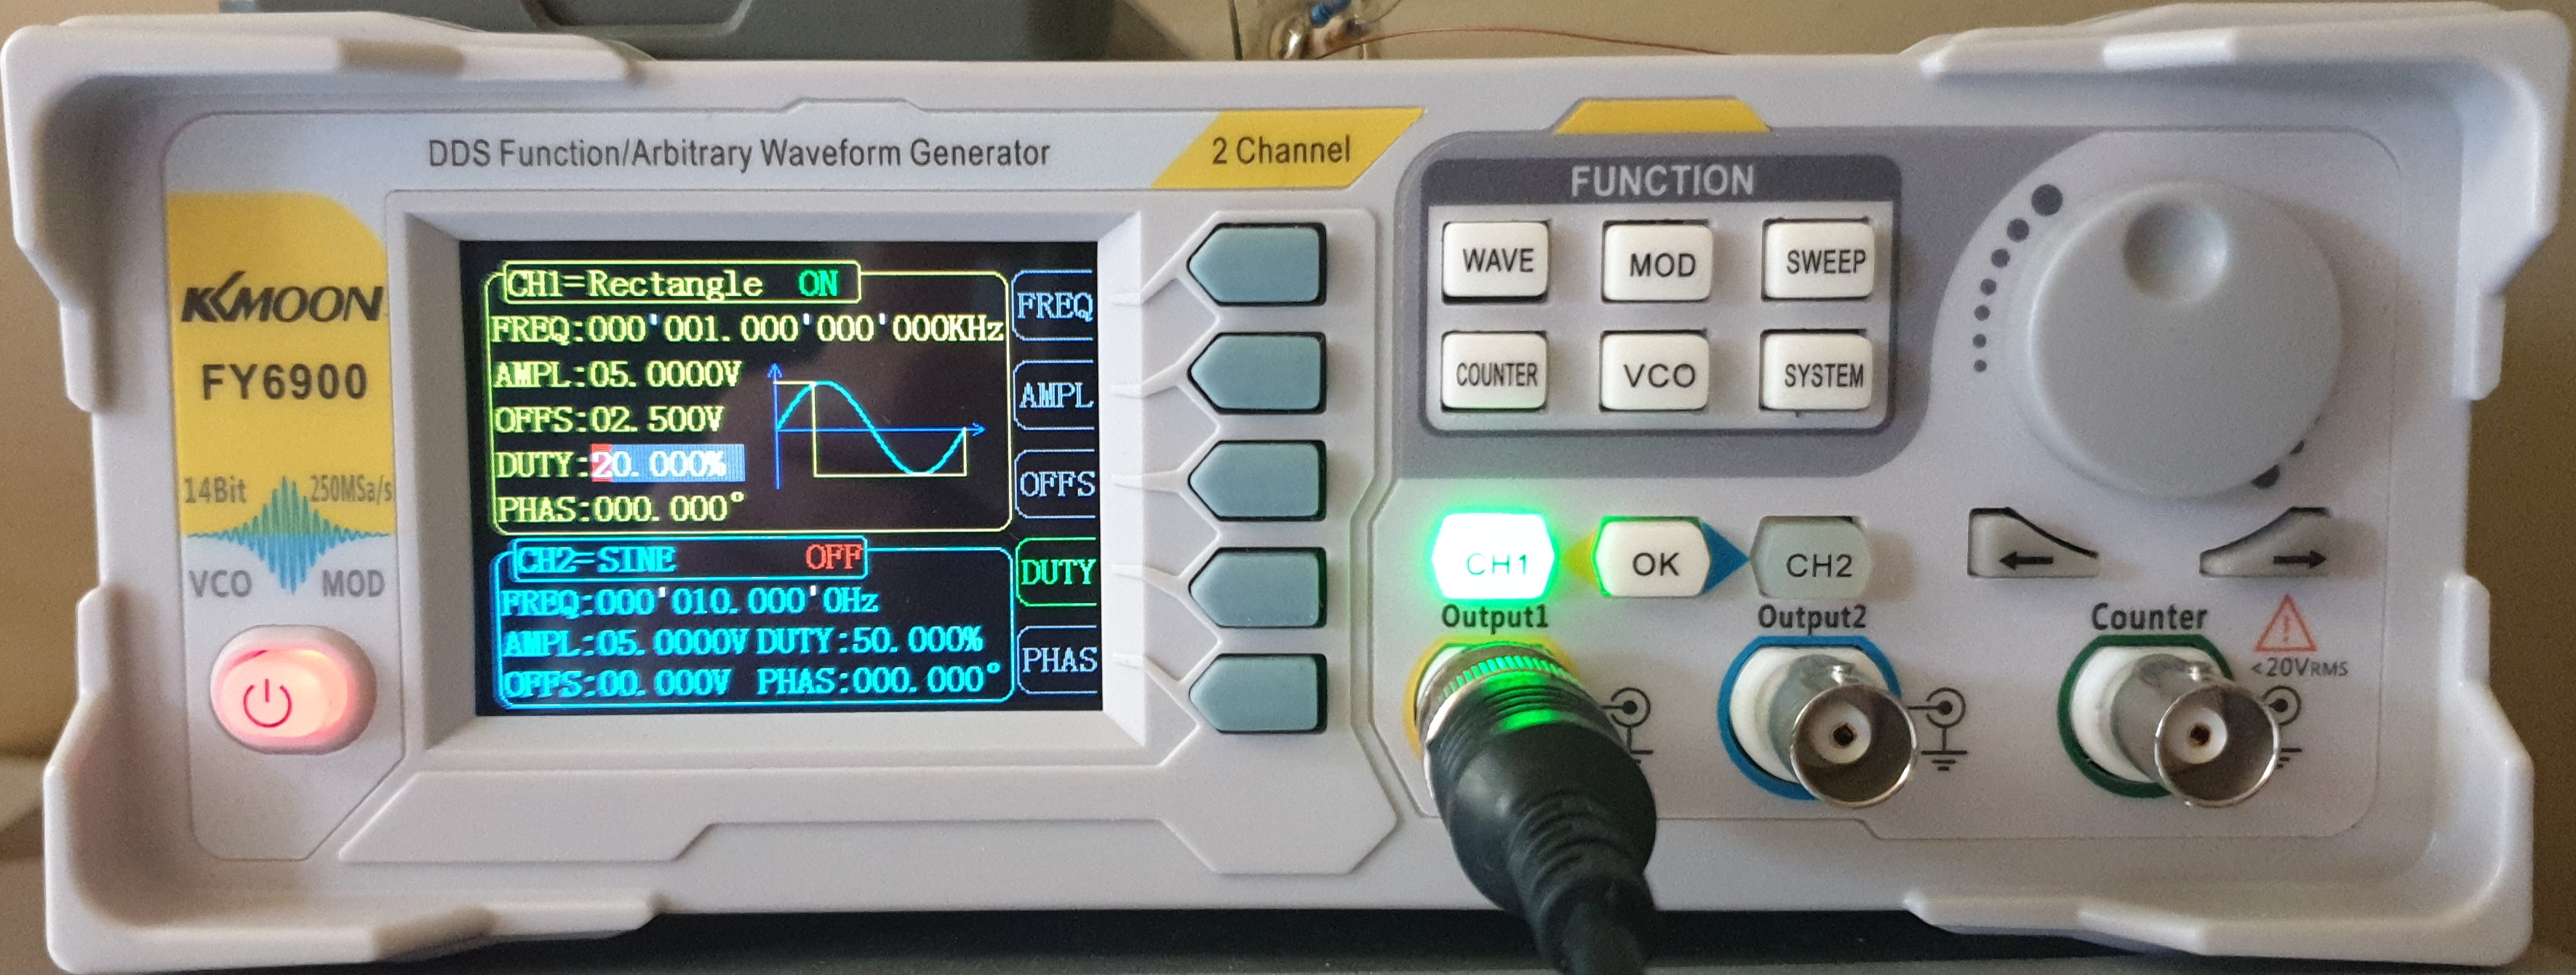
\includegraphics[width=0.80\textwidth]{ambient-linear-gen}
    \\ \vspace{5mm}
    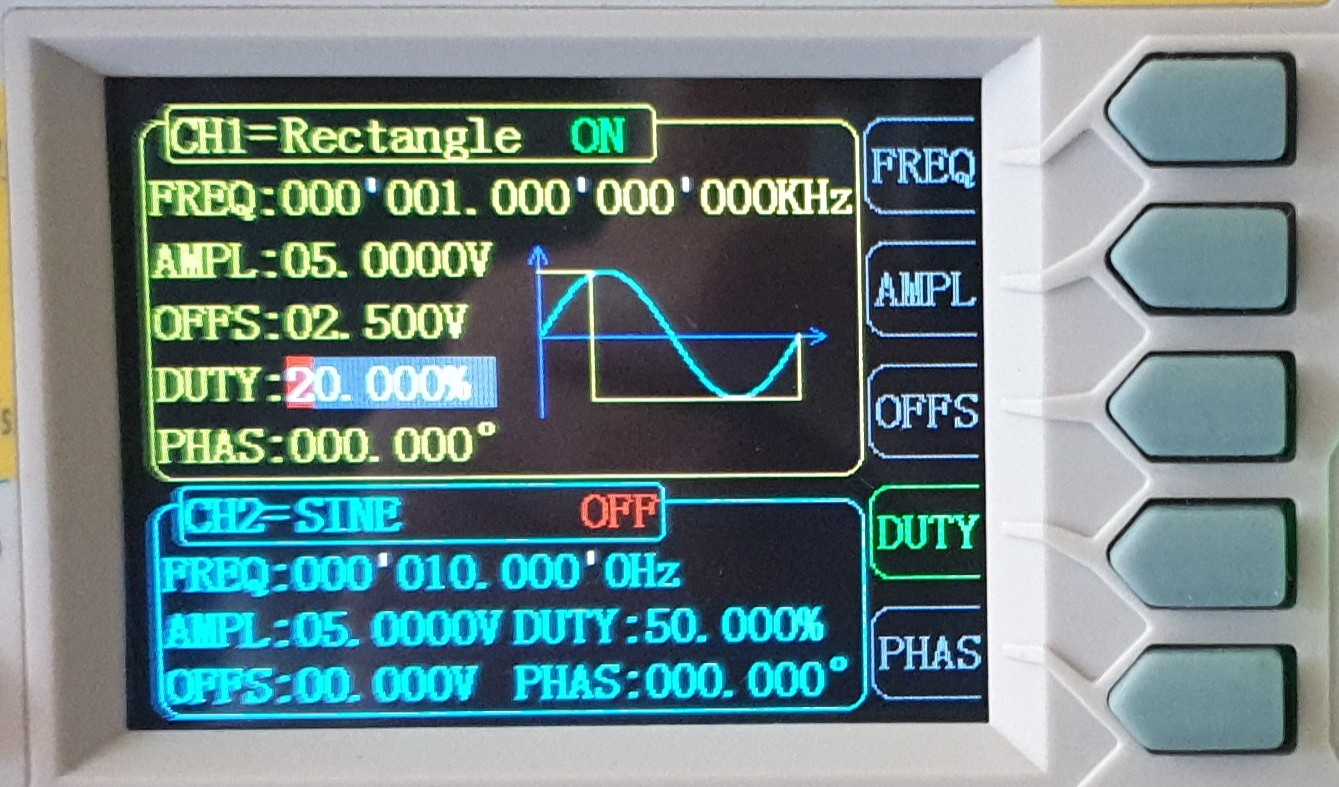
\includegraphics[height=4cm]{ambient-linear-gen-ch1}
    \hfill
    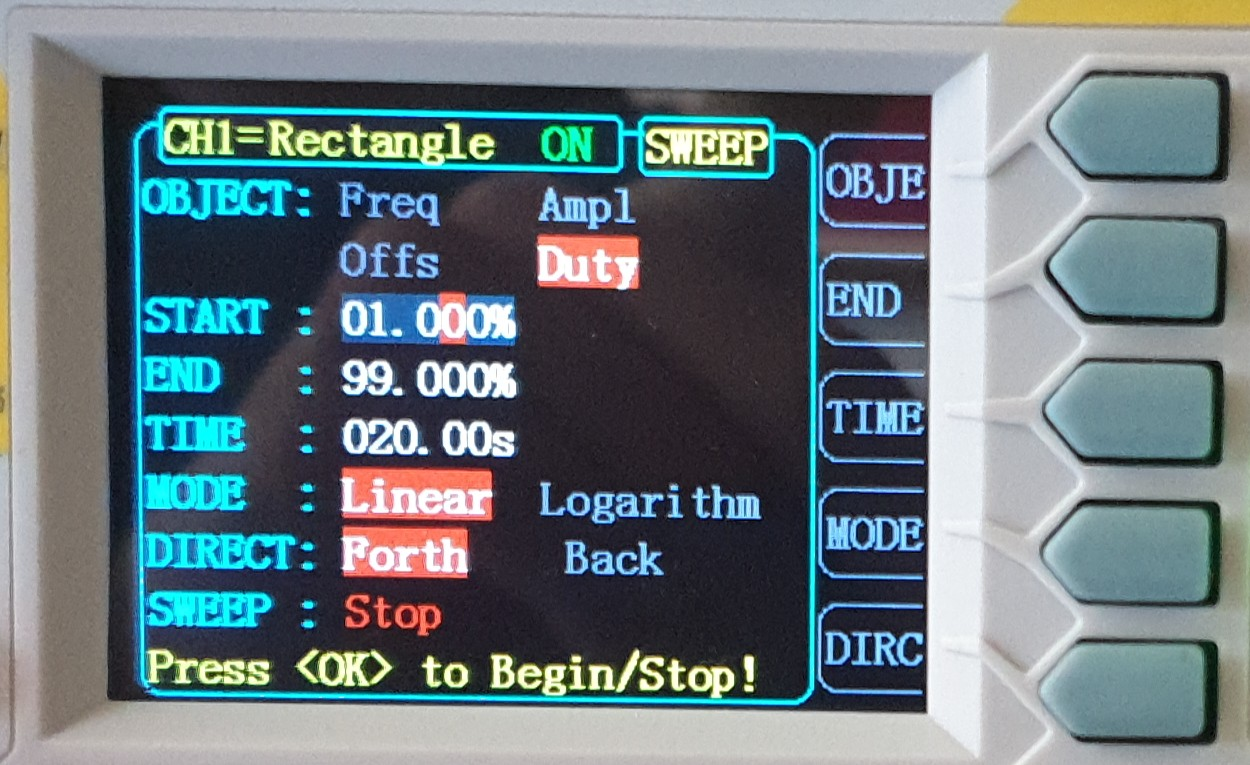
\includegraphics[height=4cm]{ambient-linear-gen-sweep}
    \caption{%
        Nastavení generátoru funkcí FY6900 pro měření závislosti proudu
        protékajícího výkonovou LED na střídě PWM signálu přiváděného na vstup
        stmívače
    }
    \label{fig:ambient linear mereni generator}
\end{figure}

K testovanému obvodu je připojen digitální osciloskop Agilent~54621A, kterým je
měřeno napětí na rezistoru R4, které je přímo úměrné proudu protékajícímu LED
diodou (proud protékající bází Q3 můžeme zanedbat). Časová základna osciloskopu
je nastavena na \SI{2}{\second}/dílek, režim spouště \texttt{NORMAL}, spouštění
na sestupné hraně použitého vstupního kanálu (na následujících snímcích
obrazovky je to kanál 2), posunutí okamžiku spuštění k levému okraji obrazovky.
Na obrazovce osciloskopu je tedy zobrazen celý průběh charakteristiky. Od
sestupné hrany signálu střída lineárně narůstá od \SI{1}{\percent} do
\SI{99}{\percent}, lze ji proto považovat za veličinu vynášenou na vodorovné
ose.

Osciloskop umožňuje uložení úplného nastavení do textového souboru na disketu:
\begin{lstlisting}[style=terminal]
Anlg Ch State  Units/Div  Position  Coupling  BW Limit  Invert
 Ch 2:    On     200mV/     600mV      DC        Off      Off

Anlg Ch Impedance   Probe
 Ch 2:    1M Ohm   1.0 : 1

Trigger  Mode   Coupling  Noise Rej  HF Reject  Holdoff
  Edge  Normal     DC         On         On       60ns

Trigger Source   Slope    Level
         Ch 2   Falling  +391mV

Time Time Ref  Main s/div  Delay
Main   Left      2.00s/     0.0s

Acquisition Realtime  Vectors  Infinite Persistence
   Normal      Off       On             Off
\end{lstlisting}

Pro porovnávání charakteristik lze navíc použít funkci digitálního osciloskopu
umožňující uložení referenčního průběhu. Ten je na obrazovce zobrazen světlejší
barvou.

Na obrázku~\vref{fig:ambient linear mereni scope dioda} jsou zobrazeny dvě
charakteristiky. Světlejší z nich je uložený referenční průběh, který byl
změřen na obvodu, ve kterém byl emitor Q1 přímo spojený se zemí. Tmavší průběh
byl změřen po zařazení diody. Pozorujeme, že dochází ke zvětšení rozsahu
regulace a prodloužení lineární části charakteristiky.

\begin{figure}[htbp]
    \centering
    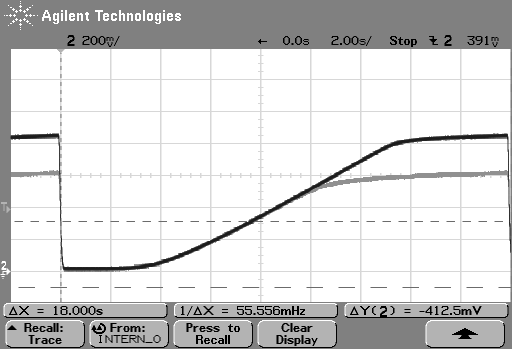
\includegraphics[width=0.80\textwidth]{scope-ambient-linear-diode}
    \caption{%
        Vliv diody připojené v propustném směru v emitoru Q1 na chování
        lineárního stmívače
    }
    \label{fig:ambient linear mereni scope dioda}
\end{figure}

\begin{figure}[htbp]
    \centering
    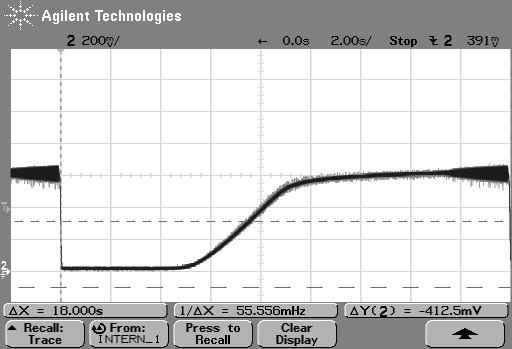
\includegraphics[width=0.80\textwidth]{scope-ambient-linear-oscillations}
    \caption{%
        Charakteristika lineárního stmívače s nevhodným průběhem a viditelnými
        oscilacemi
    }
    \label{fig:ambient linear mereni scope oscilace}
\end{figure}


% Schema z KiCAD. Zatim ho sem davat nebudu, melo by jine refdes apod.
%\begin{figure}[htbp]
%    \centering
%    %\includegraphics[width=0.9\textwidth]{cropped_ambient-linear-prod}
%    \caption{%
%        Schéma zapojení konečné verze lineárního stmívače pro výkonovou LED}
%    \label{fig:ambient linear prod sch}
%\end{figure}
